\section{Conformal Invariance}
\label{ch:conf}

Lorem ipsum dolor sit amet, consectetur adipisicing elit, sed do eiusmod tempor
incididunt ut labore et dolore magna aliqua. Ut enim ad minim veniam, quis
nostrud exercitation ullamco laboris nisi ut aliquip ex ea commodo consequat.
Duis aute irure dolor in reprehenderit in voluptate velit esse cillum dolore eu
fugiat nulla pariatur. Excepteur sint occaecat cupidatat non proident, sunt in
culpa qui officia deserunt mollit anim id est laborum.

\begin{figure}
\begin{center}
    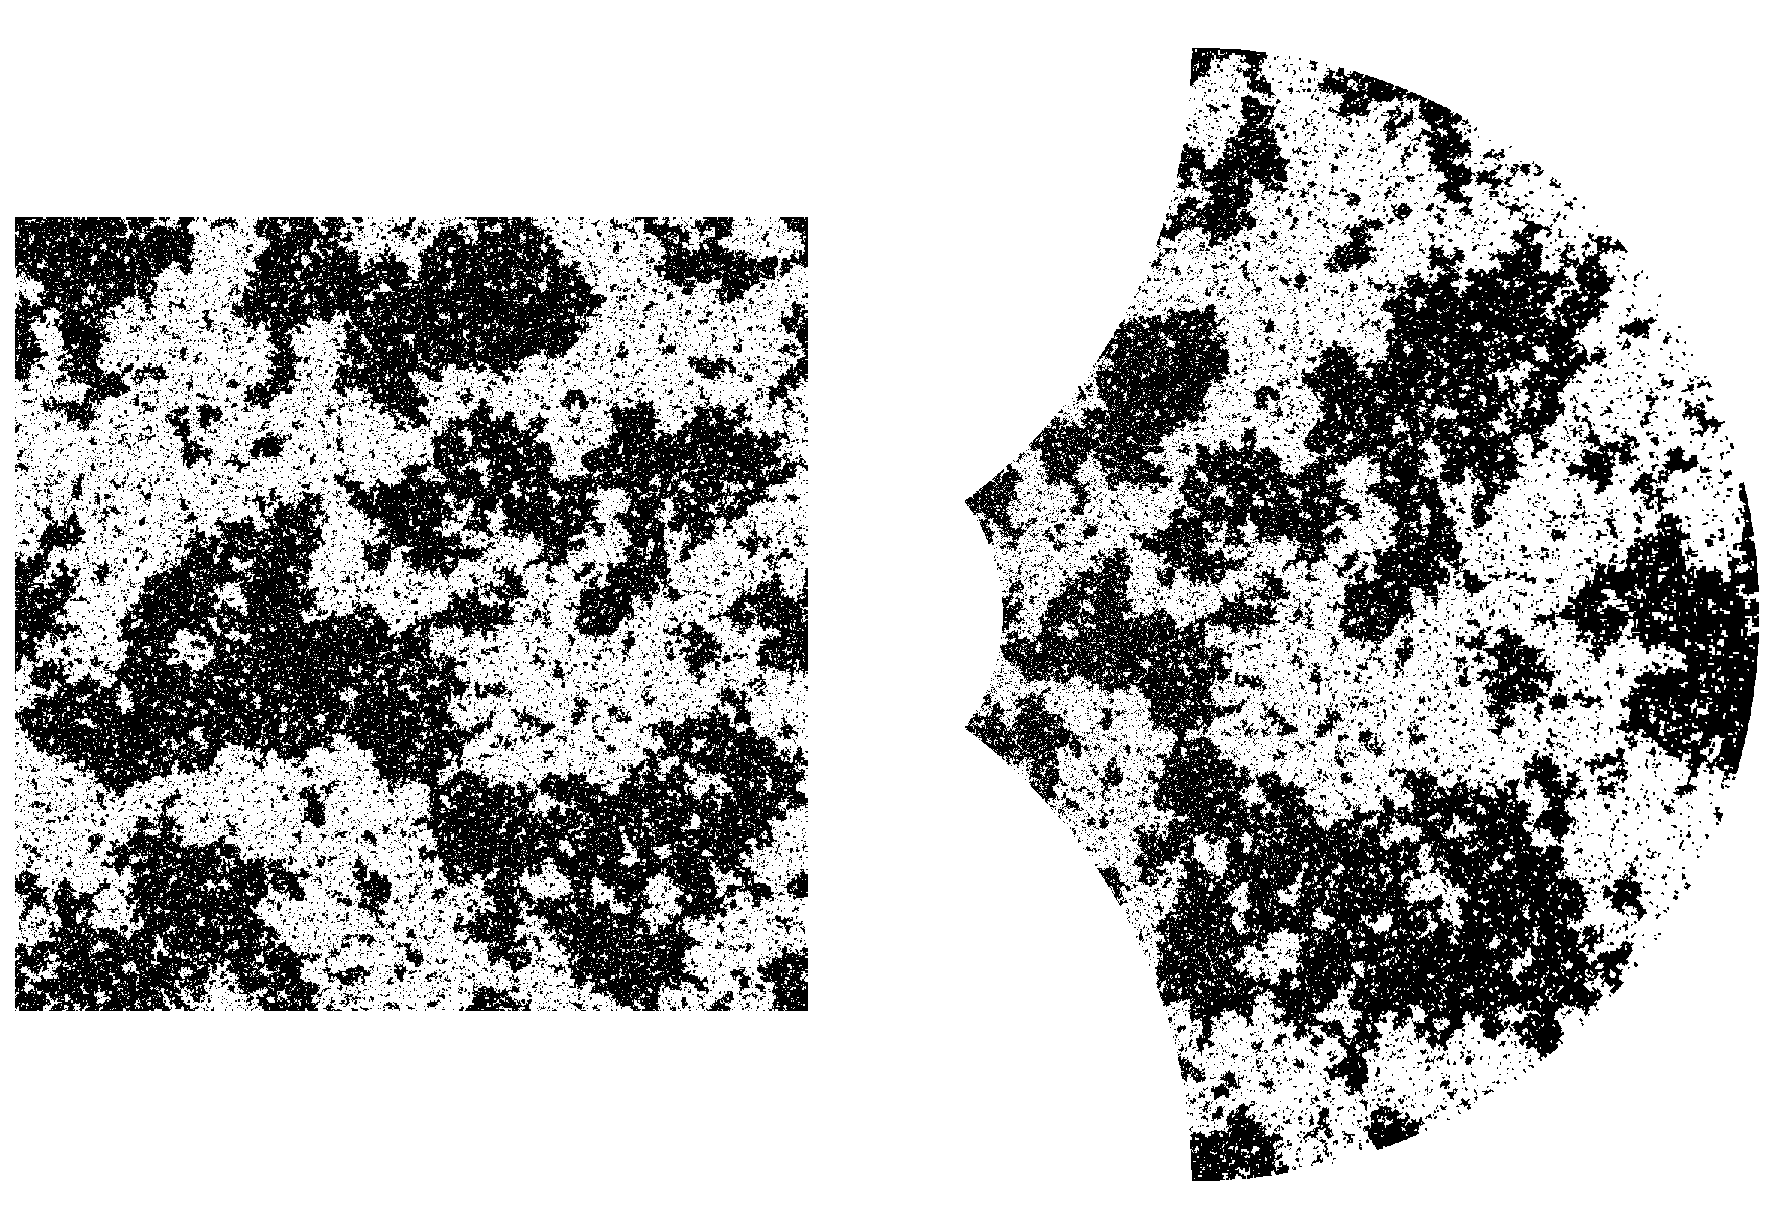
\includegraphics[scale=0.4]{chapters/ch3-conf/figs/isingcm}
\end{center}
\caption{Illustration of the Ising model at the critical point when transformed
    under a conformal map $f(z)=z/(2-z)$. The deformed image still looks
    statistically similar to the original, which is a consequence of conformal
    invariance.}
\label{fig:isingcm}
\end{figure}

\begin{figure}
\begin{center}
    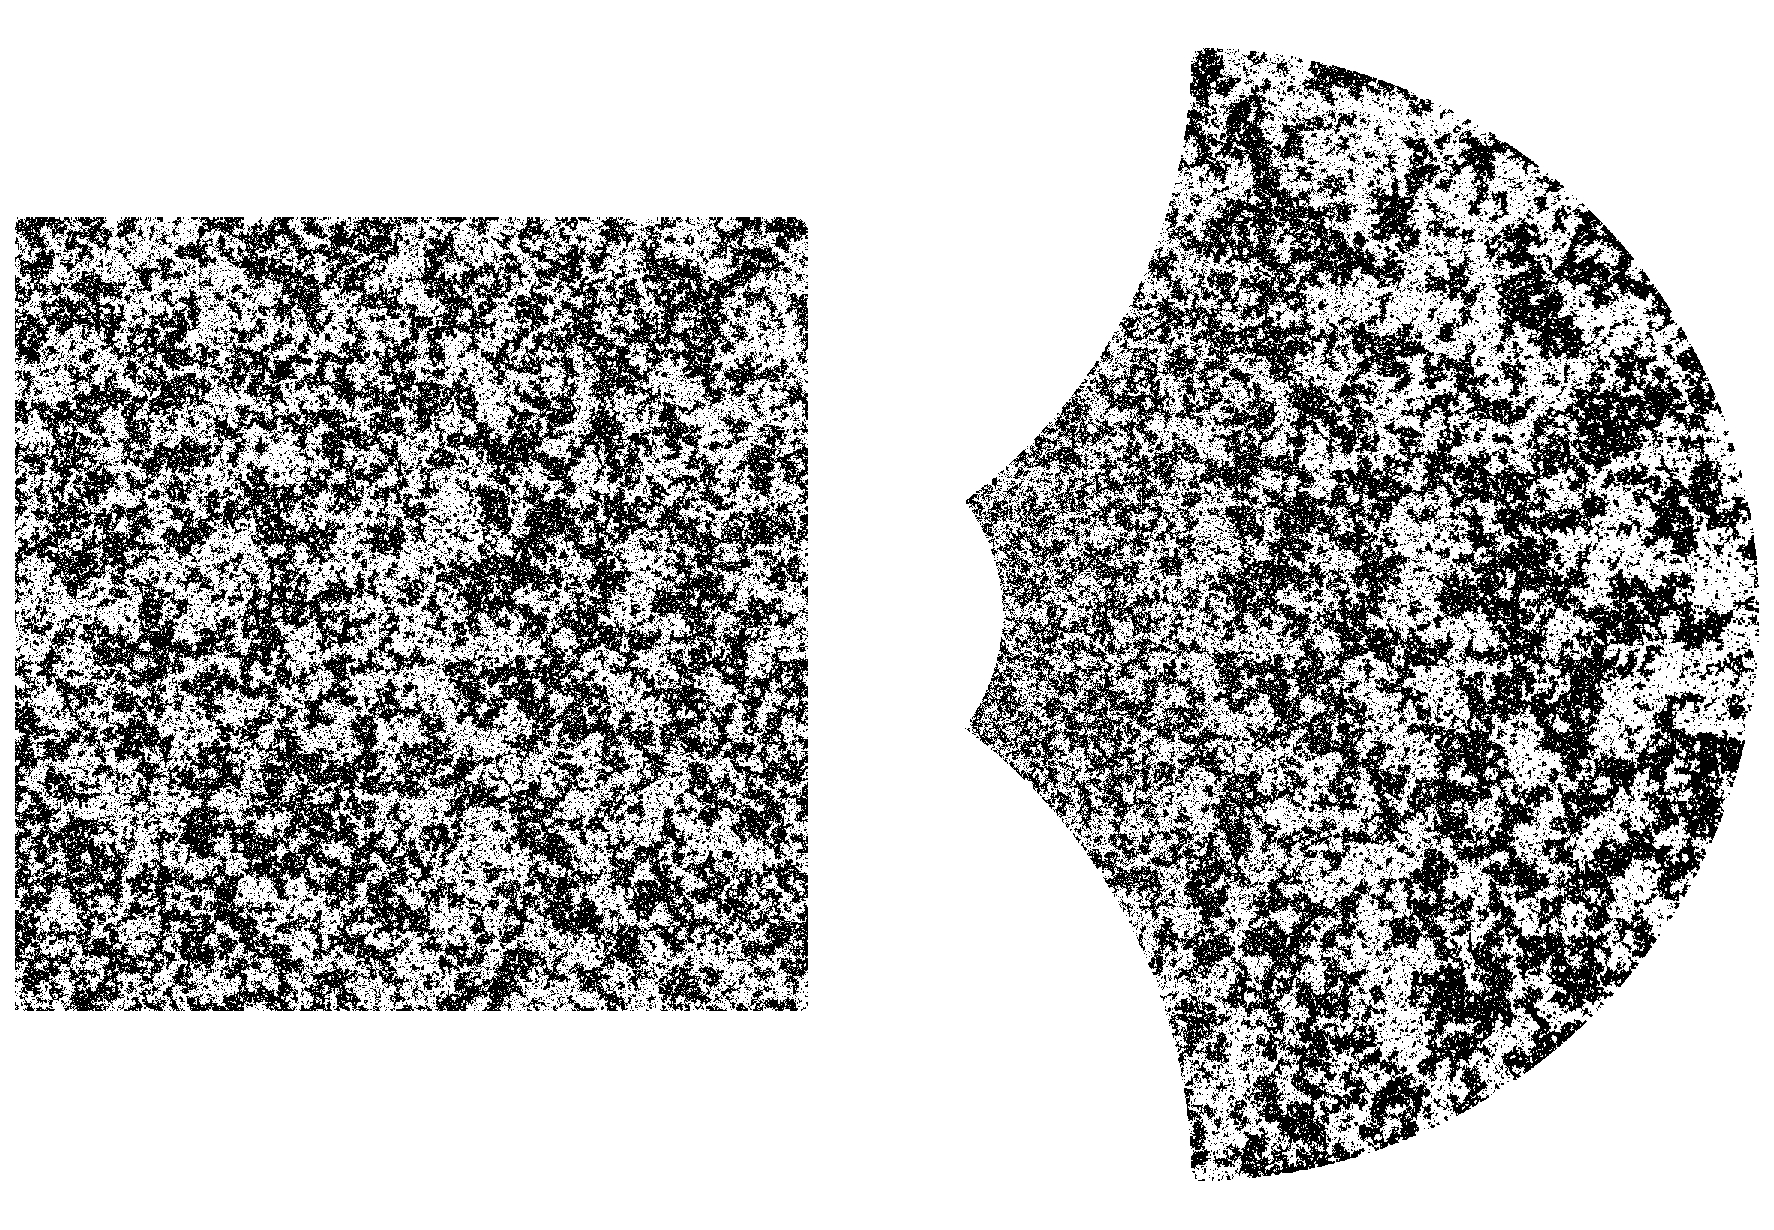
\includegraphics[scale=0.4]{chapters/ch3-conf/figs/isingcm2}
\end{center}
\caption{Illustration of the Ising model above the critical point when
    transformed under a conformal map $f(z)=z/(2-z)$. In the deformed image,
    the spin configuration is no longer homogeneous, because outside the
    critical point the system is no longer conformally invariant.}
\label{fig:isingcm2}
\end{figure}
